\chapter{Experiments [SP]}
\label{chap:experiments}
The goal of our work is to compare two implementations of the Speed layer, one using Storm and another using Spark Streaming.
We evaluate both approaches from two sides.
First, we measure the performance of the system to detect which techology allows to process more events for the specified time interval.
Second, we compare the codability of these variants.
Using the obtained results, we make a choice which technology fits better our case.

\section{Performance Evaluation}

Figure~\ref{fig:test_system_parameters} represents the parameters of the test system.
For the simplicity of testing we use only one machine.
To obtain more reliable results one should also test these systems on a cluster of several machines.

\begin{figure}[h]
  \centering
  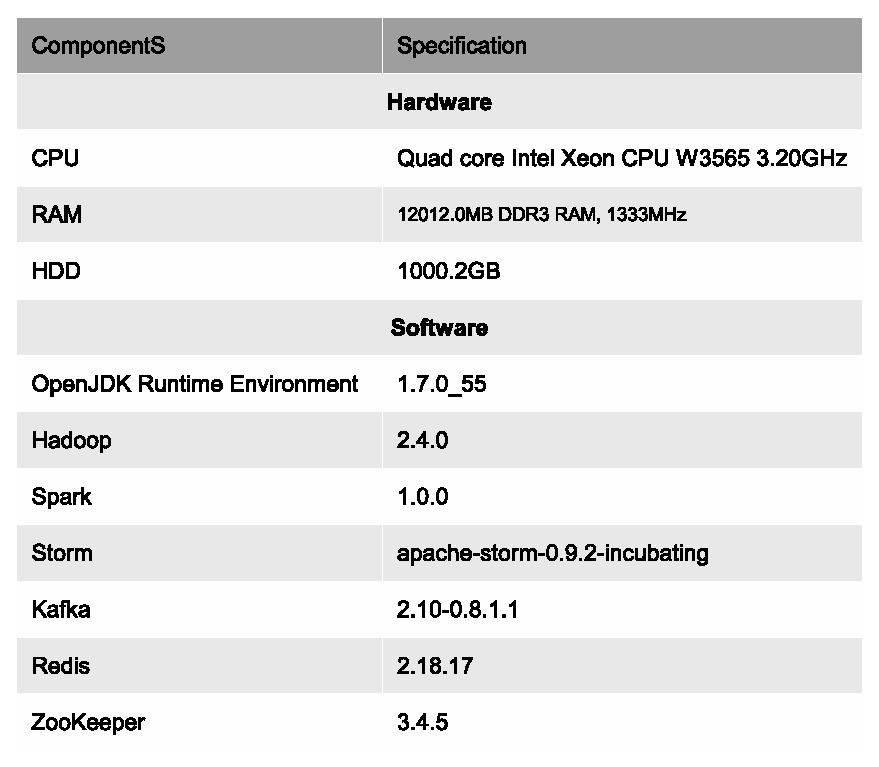
\includegraphics [width=0.9\textwidth]{images/test_system_parameters}
  \caption{Test system parameters}
  \label{fig:test_system_parameters}
\end{figure}

As an input, we use automatically generated events, that imitate the real data flow.
To make the comparison more objective, we vary the number of processed messages.
In our tests we use three sets: \textit{1,000} events, \textit{10,000} events and \textit{100,000} events.
Each of these sets contains all types of events mentioned in Chapter 8.
The values of event parameters are generated randomly.

As an output, we obtain the speed of event processing.
We measure how much time it takes to process the fixed amount of events and compare these figures for both Storm and Spark implementations.
The vertical axis of all 3 diagrams below is the time in milliseconds.
The horizontal axis represents the number of processed events.

As we can see, in all cases graphic increases almost linearly.
It is obvious that the more events we want to process the more time we need.
Furthermore, the system processes the fixed number of events in approximately the same time interval.
It gives the possibility to estimate the overall time needed to handle the specified number of events, measuring the time expenditure for a small part of the whole set.

\begin{figure}
  \centering
  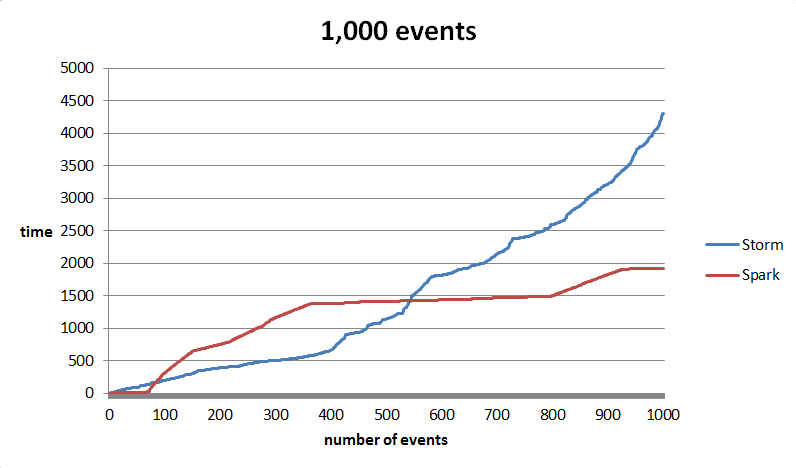
\includegraphics [width=1.0\textwidth]{images/exp1}
  \caption{Processing 1,000 events}
  \label{fig:1000events}
\end{figure}

\begin{figure}
  \centering
  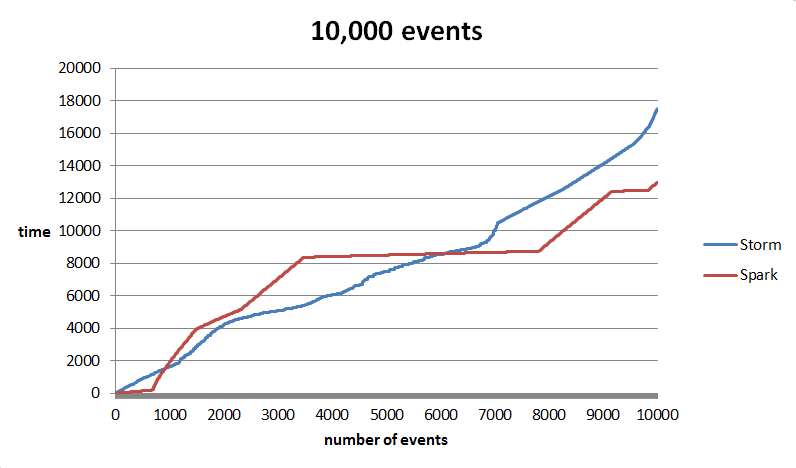
\includegraphics [width=1.0\textwidth]{images/exp2}
  \caption{Processing 10,000 events}
  \label{fig:10000events}
\end{figure}

\begin{figure}
  \centering
  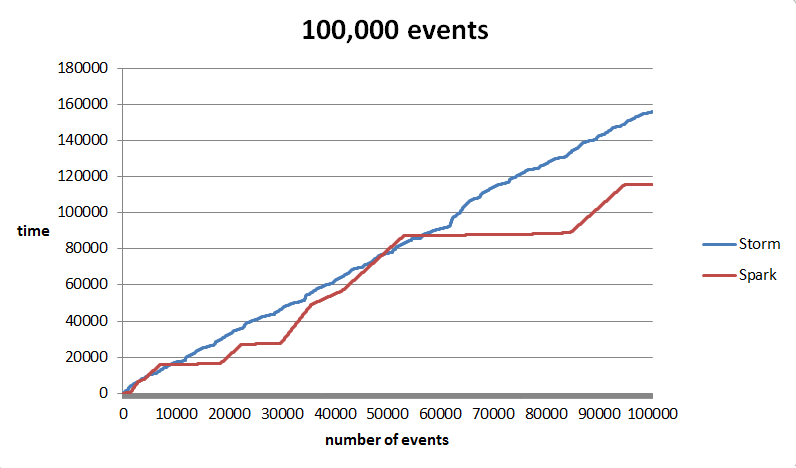
\includegraphics [width=1.0\textwidth]{images/exp3}
  \caption{Processing 100,000 events}
  \label{fig:100000events}
\end{figure}

It is clearly shown on diagrams, that Strom and Spark have different processing techniques.
Storm performs indeed a real time processing.
Its graphic, especially for the \textit{100,000} events case is close to a straight line.
Spark, in its turn, does a micro-batching.
The size of batch is small, so this technology can be considered close to real time processing.
However, as we look at processing in milliseconds scale, we can see obvious steps on Spark diagrams. 
We expected to have straight steps of equal size, but in our case they a bit skew and have different size.
This can happen because of the several reasons.
For example, the system setting (batch size, etc.) can be not optimal for our case, so Spark works with delays.
Or we can have an inaccuracy in our measurements, or the measurement supplements can distort the processing routine.    

As a conclusion, we can say that on every scale - \textit{1000}, \textit{10,000} and \textit{100,000} - events Spark processes events faster than Storm.
The only disadvantage of Spark is that it cannot give the true real-time processing.
Even if the size of batch in micro-batching technique is small, it still cannot guarantee the immediate result.
In our case this delay is not critical, however in other applications this technique can be not feasible because of this reason.  

\section{Codability}

In the previous section Storm and Spark implementations are compared from the performance point of view.
However, it is not the decisive factor when choosing which technology to use in our project.
In modern world the cost of hardware decreases significantly comparing to the prices that were ten years ago.
Thus it is not a problem to add several machines into our cluster, increasing performance.
Hence the human sources become an important factor for making our choice.
In this section we compare which technology, Storm or Spark, is easier to implement.

\mnote{installation}
The installation process of Storm is a bit more complicated than the installation of Spark.
Storm requires two additional tools to be installed on a machine.
First, it needs ZooKeeper for coordinating the cluster.
Second, Strom should run under supervision, so a supervisor service like a \textit{supervisord} is needed.
From the practical side we had some difficulties with combining the versions of these software tools to make them interact properly.
Spark, in its turn, only requires a Spark assembly in the CLASSPATH.

\mnote{configuration}
Storm and Spark have different configuration settings to integrate with Kafka.
To allow Kafka-Storm interaction, we use an existing storm-kafka module.
It provides a special class \textit{KafkaSpout}, that receives data from Kafka.
As Kafka and Storm interact through ZooKeeper, we specify ZooKeeper hosts, port and a path to Kafka brokers (clusters).
Furthermore, each Kafka spout stores consumer offsets in ZooKeeper.
For this purpose we specify a root path in ZooKeeper and a unique id for every spout.
There is a possibility to set from which offset to start consuming.
Also we indicate a topic name for each spout.
To provide Spark with the data from Kafka, the following settings are needed.
We specify a list of ZooKeeper hosts, the name of Kafka consumer group and the topic name.
The number of threads used for consuming data from a Kafka topic is also customizable.

\mnote{usage}
From our subjective point of view, the process of implementation is more intuitive for Storm comparing to Spark.
The idea that data goes from source to spouts, from spouts to bolts is very transparent.
It is easy to design a system architecture and implement its components.
For Spark it is more complicated.
One has to understand the concept of RDD, the difference between transformations and actions.
We should take into account that when we run transformations on RDD, the transformation code is serialized, shipped to the node and deserialized.
Hence we have to provide serializable classes, that complicates the implementation process.

\mnote{documentation}
Both Spark and Storm have an official online documentation available.
They have a good description of the general usage.
The Storm website provides a link to an example project named \textit{storm-starter} that can be used as a basis for creating your own project.
Spark package also contains an example project, that includes \textit{JavaKafkaWordCount.java} code, that can be used as a starting point. 
The only distinction that should be mentioned is the availability of documentation about integration with Kafka.
As the support of Kafka was included only in the last version of Storm (storm-kafka-0.9.2-incubating), this module is not wholly documented and there are no examples on the official Storm site.
On the contrary, Spark has an example code on its official site and API documentation. 

\mnote{community size}
Another important factor is a community size of the project.
Documentation is a good source of information, however in cannot cover all the questions that can appear during the development process.
People who work on a project are the most competent sources, they can answer unusual questions and help providing code examples.
Moreover, they can determine that the unexpected behavior of the system is a bug and promote a solution.
We can compare the number of contributors of Spark and Storm using github statistics, because both these projects present there.
Currently Spark has 355 contributors, while Storm has 115 contributors. 

\begin{figure}[h]
  \centering
  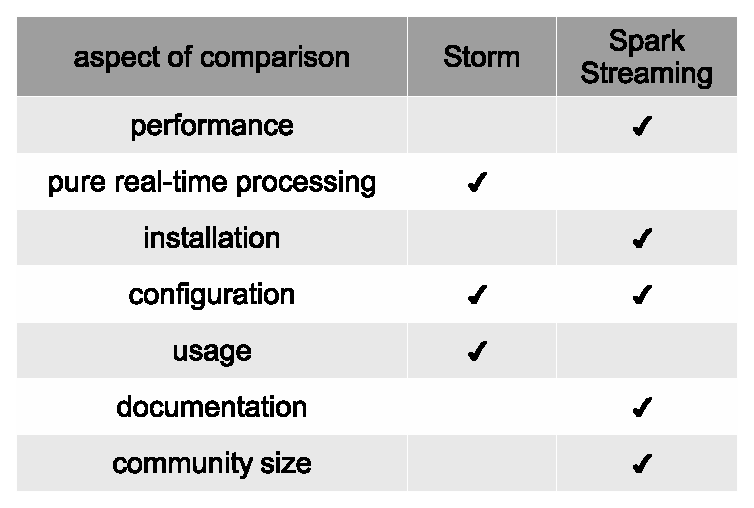
\includegraphics [width=0.6\textwidth]{images/storm_spark_comparison}
  \caption{Summarizing comparison of Storm and Spark Streaming implementations}
  \label{fig:storm_spark_comparison}
\end{figure}

To summarize the aspects of Storm and Spark Streaming comparison we present the concluding table shown in Figure~\ref{fig:storm_spark_comparison}.
The checkmark in one of the column means that the specified aspect of a specified technology gives better results than the competitor.
If both columns contain a checkmark it means that this aspect is equal for both technologies.

It should be mentioned that the comparison of Storm and Spark Streaming as separate technologies is not our goal.
We want to choose the technology that can be used to build a Speed layer of Lambda architecture in the context of the Menthal project.
Looking at the summarizing table we can conclude that Spark has more advantages than Strom.
Hence, for our purposes the Spark Streaming approach appears to be the best solution.